\begin{center}
    \textbf{--------- lezione 2 - 3 marzo 2021 ---------}
\end{center}
\section{Architettura di un sistema}
Principalmente si parla di architetture software e hardware. Un'architettura di un sistema distribuito definisce:
\begin{itemize}
    \item le entità principali del sistema
    \item i pattern della comunicazione (client-server, event-bus o pub/sub, peer-to-peer)
    \item come comunicano (modi con i quali i processi in esecuzione su macchine disclocate in posti diversi comunicano)
    \item ruolo delle entità (client o server) e come possono evolvere (client diventa server e poi magari ritorna anche client)
    \item come le entità sono mappate a livello di infrastruttura fisica (potrebbero essere replicati)
\end{itemize}

\section{Architetture centralizzate}
Le due architetture centralizzate più note sono:
\begin{itemize}
    \item Client-server (basato su una richiesta e una risposta)
    \item Event bus (basato su eventi che utilizza publish subcribe)
\end{itemize}

\subsection{Client Server}
\begin{center}
    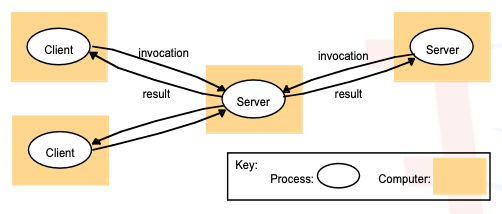
\includegraphics[width = .6\textwidth]{images/lezione2/cs-schema.png}
\end{center}
Abbiamo dei processi sui nodi, i clients invocano una richiesta al server che deve gestire più richieste e deve rispondere a tutti quanti. In questo schema c'è un solo server, ma nella realtà potrebbero essercene più di uno.
\begin{center}
    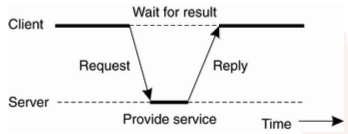
\includegraphics[width = .6\textwidth]{images/lezione2/CS.png}
\end{center}
In questo grafico si ha sull'asse delle ascisse lo scorrere del tempo. La linea marcata rappresenta un processo in esecuzione, la linea tratteggiata indica un processo che o non è in esecuzione o sta facendo altro (ad esempio il server potrebbe servire un altro client e il client va in wait in attesa della risposta).
L' inclinazione delle frecce di richiesta/risposta sono oblique perché c'è sempre un delay temporale di comunicazione da tenere in considerazione.

\begin{center}
    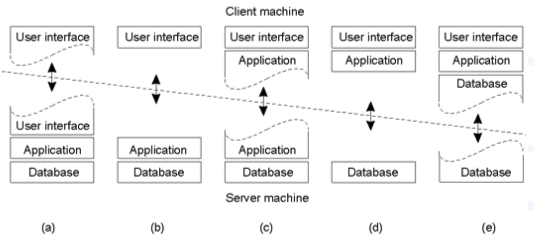
\includegraphics[width = .7\textwidth]{images/lezione2/bilanciamento.png}
\end{center}
Cosa esegue il server e cosa il client?\\
Dobbiamo scegliere in fase di progettazione.
Possiamo andare a caricare o scaricare il client e il server in base al tipo di componenti che stiamo utilizzando. 

\begin{center}
    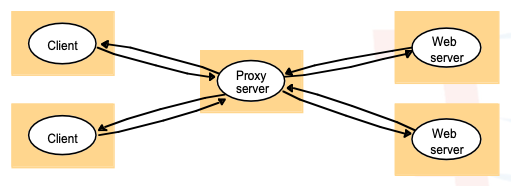
\includegraphics[width = .7\textwidth]{images/lezione2/caching.png}
\end{center}
Possiamo fare uso di sistemi di caching ad esempio tramite l'utilizzo di proxy server che fanno anche questo servizio. \\
Il funzionamento è molto semplice: quando viene fatta una richiesta che era già stata fatta recentemente e viene valutato che la risposta alla richiesta è uguale a quella di prima (è ancora fresca) non si va a disturbare ancora il server ma si utilizza un proxy server che ha tenuto in cache la risposta data precedentemente.

\begin{center}
    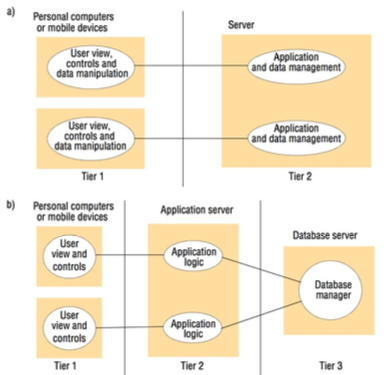
\includegraphics[width = .5\textwidth]{images/lezione2/multitier.png}
\end{center}
Esistono architetture client-server definite come multitier (multi livello). In queste si aggiunge la gestione di più livelli lato server. In un interazione con il client divido le funzionalità lato server in più livelli ad esempio application server e database server. \\
Quando parliamo di server multi livello non sempre intendiamo due macchine diverse, possiamo intendere anche due processi diversi sulla stessa macchina.

\subsubsection{Distribuzione}
Esistono diversi tipi di distribuzioni che non sono altro che modi per distribuire il carico di lavoro e rendere efficienti i sistemi distribuiti. Le principali sono:
\begin{itemize}
    \item distribuzione verticale: si ha un server (inteso non per forza come macchina fisica) differente per ogni funzionalità
    \begin{center}
        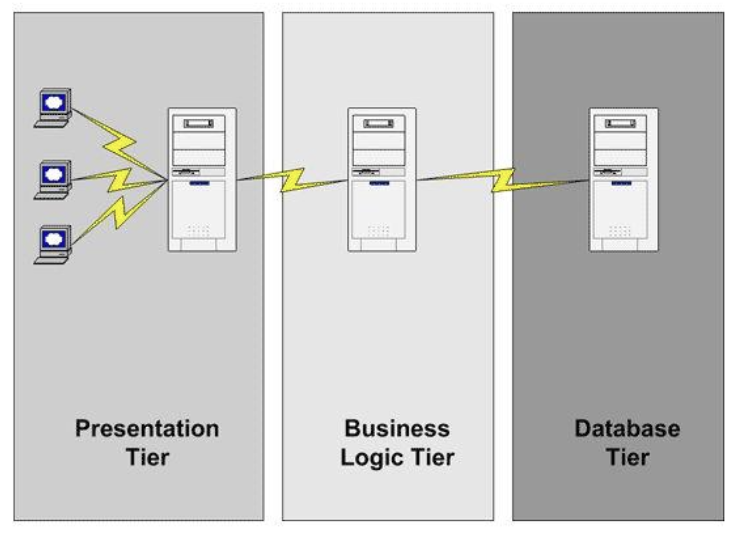
\includegraphics[width = .4\textwidth]{images/lezione2/vert-dist.png}
    \end{center}
    \item distribuzione orizzontale: si ha una stessa funzionalità distribuita (replicata) su nodi diversi
    \begin{center}
        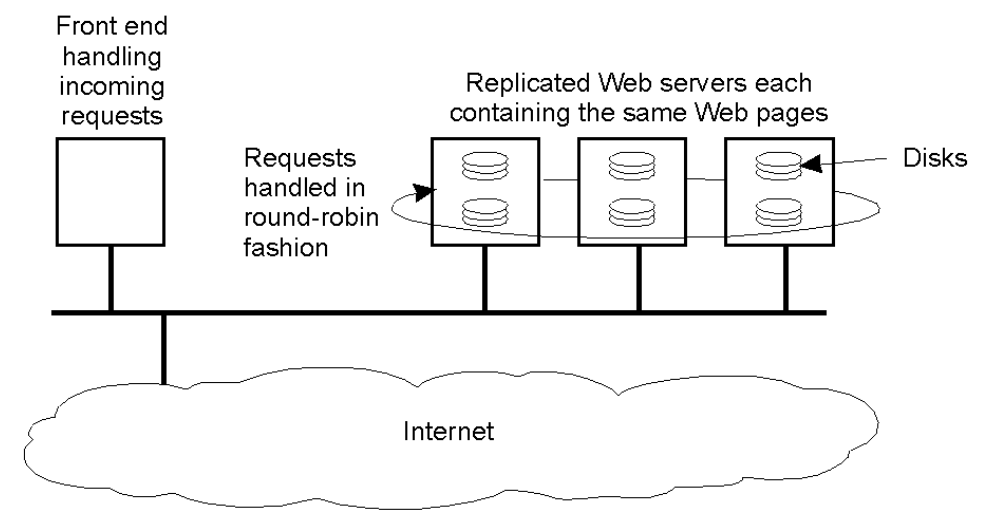
\includegraphics[width = .6\textwidth]{images/lezione2/or-dist.png}
    \end{center}
    \item distribuzione combinata: ogni funzionalità è duplicata su un gruppo di server. In questa distribuzione abbiamo il load balancer che si occupa di smistare il carico di lavoro.
    \begin{center}
        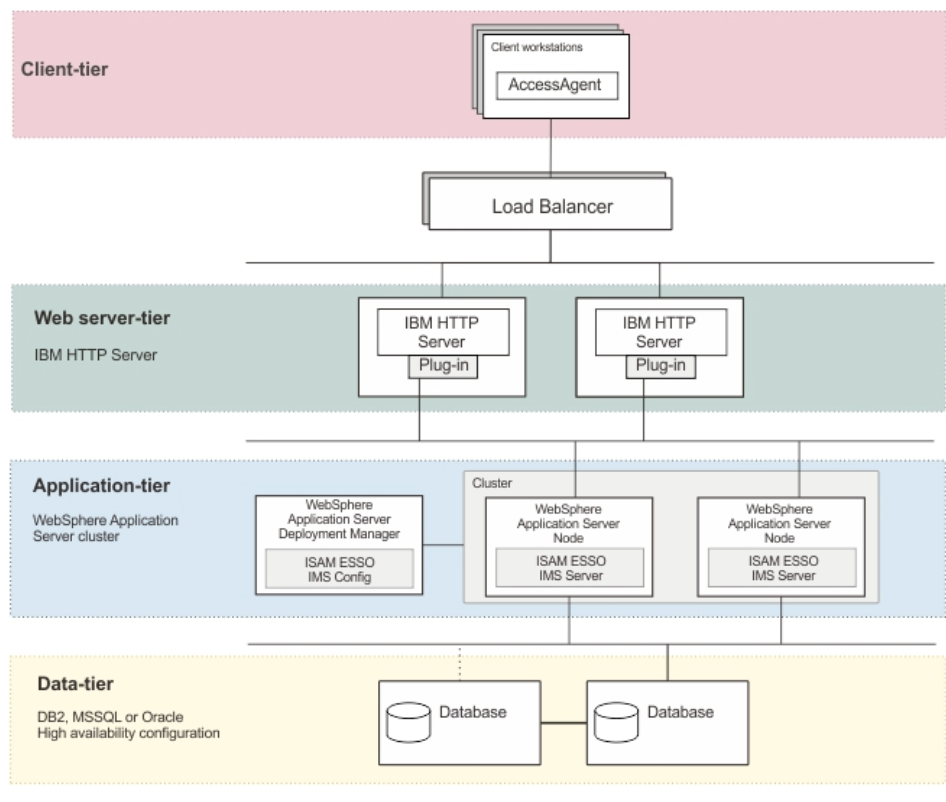
\includegraphics[width = .5\textwidth]{images/lezione2/vert-or-dist.png}
    \end{center}
    
\end{itemize}

\subsection{Event Bus architecture}
È un tipo di architettura molto utilizzato nell'ambito iot.
    \begin{center}
        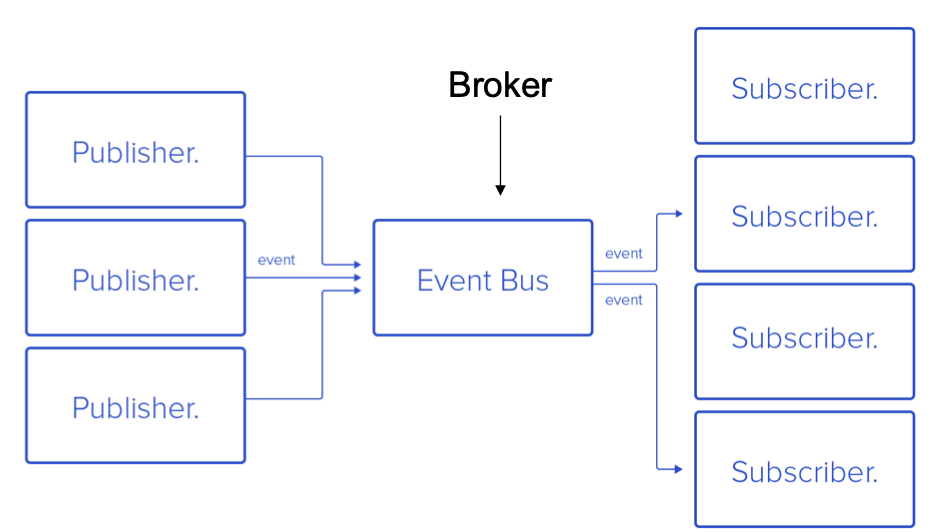
\includegraphics[width = .5\textwidth]{images/lezione2/eventbus.png}
    \end{center}
In questa architettura abbiamo tre diverse componenti:
\begin{itemize}
    \item broker: è un componente software che gestisce l'event bus.
    \item publisher: client che comunicano che si è verificato un aggiornamento. Esempio: in questa stanza è stato registrato un cambio di temperatura di 1 grado
    \item subscriber: si "iscrive" a ricevere tutti gli aggiornamenti di uno o più publisher. Esempio: aggiornamenti sui cambi di temperatura.
\end{itemize}
Il broker quindi ha il compito di comunicare ai subscriber interessati gli eventi registrati dai publisher.

\section{Architetture decentralizzate}
\subsection{Peer-to-peer}
\begin{center}
    \includegraphics[width = .4\textwidth]{images/lezione2/P2P.png}
\end{center}
Abbiamo diversi peer (nodi), dove ognuno ha le stesse capacità funzionali degli altri. È un'architettura disegnata in modo che ogni peer abbia risorse condivisibili. Non c'è il coordinatore (load balancer), ma i nodi sono tutti alla pari.
\begin{center}
    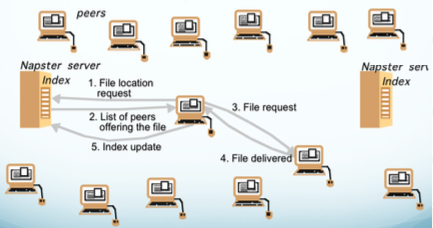
\includegraphics[width = .6\textwidth]{images/lezione2/napster.png}
\end{center}
Un esempio di architettura P2P è quello di Napster che è stato il primo sistema che ha dimostrato utilità e efficacia di un sistema distribuito su larga scala per lo scambio di risorse che sono file. È nato più di vent'anni fa ed è stato chiuso per questioni di copyright. \\
Questo sistema non era peer to peer puro. Come possiamo vedere dallo schema c'è un napster server che mantiene un index. Tutti i nodi hanno sia funzionalità di client e di server ed eseguono tutti lo stesso codice, tranne appunto i server "direcory". \\ La gestione degli indici è centralizzata. Se un client vuole un certo file, manda richiesta al server iniziale che risponde con una lista di indirizzi di peer che dovrebbero avere quel file. Il peer a questo punto usa uno di questi indirizzi e contatta un altro peer, che si comporta da server. Se ha il file lo restituisce al client (quello che fa la richiesta) come risposta. Il client dice all'indice di aggiornarsi in modo che si tenga traccia che anche lui adesso ha il file. Viene quindi reso disponibile il file su più punti della rete P2P.\\\\

Uno dei problemi principali delle architetture P2P è capire come distribuire le risorse. Gli obiettivi nel distribuire sono:
\begin{itemize}
    \item raggiungere load balancing quando si accede ai dati, migliorare quindi le performance
    \item assicurare disponibilità, proteggersi quindi da eventuali guasti
    \item evitare troppi overhead
\end{itemize}

\subsubsection{Generazioni di sistemi P2P}
\begin{itemize}
    \item Prima generazione: primi sistemi di condivisione di file. \\
    Esempio: Napster.
    \item Seconda generazione: vengono migliorati i protocolli per aumentare scalabilità, fault tolerance e anonimità. \\
    Esempi: 
    \begin{itemize}
        \item Gnutella: tentativo di fare un sistema puro che funziona su larga scala, non usa directory service completi e che ha indici parziali e distribuiti.
        \item FreeNet: aveva come obiettivo quello di fornire file sharing che garantisse anonimità.
        \item bitTorrent: particolarmente efficiente per una caratteristica fondamentale: non viene scambiata la risorsa intera, ma vengono gestiti diverse porzioni di file.
    \end{itemize}
    \item Terza generazione: viene introdotto il P2P Middleware, un sistema che è una specie di middleware per gestire in modo distribuito e decentralizzato delle risorse.
\end{itemize}

\subsubsection{Obiettivi del Middleware P2P}
Deve abilitare i client a poter:
\begin{itemize}
    \item localizzare e comunicare con una risorsa
    \item aggiungere e rimuovere risorse
    \item aggiungere e rimuovere peers
\end{itemize}
in modo completamente trasparente.\\
Per poter raggiungere questi obiettivi si costruiscono le overlay networks.

\subsubsection{Overlay Network}
Rete logica (virtuale) costruita sopra la vera rete (fisica) che collega i peer. \\
Criteri di ottimizzazione: scalabilità, load balancing, far comunicare i peer vicini (minore latenza), sicurezza e anonimità. Questa rete logica consente di effettuare in modo efficiente le cose suddette. 
Sulla rete logica viene seguito il routing delle richieste (a livello applicazione) da client magari anche esterni alla rete agli host/nodi che contengono le risorse che ci interessano). Non è il routing del protocollo IP, è routing a livello di applicazione. È basato non su indirizzi IP, ma su identificatori globali. Le risorse hanno identificatori globali nel sistema distribuito. Il routing deve instradare verso uno dei peer che hanno una replica della risosa (quindi possono averla più di uno). I protocolli di routing overlay devono anche occuparsi di inserire e rimuovere nodi e oggetti. Questo algoritmo è installato su tutti i nodi del sistema. \\
Esistono essenzialmente due tipi di overlay network:
\begin{itemize}
    \item strutturate: sono le più utilizzate oggi. Danno garanzie maggiori. In queste reti c'è un algoritmo deterministico con strutture dati particolari per cercare all'interno di questa rete logica (spesso viene gestita tramite tabelle di hashing).
    \item non strutturate: usano algoritmi probabilistici/randomizzati. Ogni peer non sa esattamente dov'è nella rete logica. Ha una vista parziali di alcuni altri peer che si evolve nel tempo. Siccome è parziale, nel momento in cui un client fa una richiesta a uno di questi peers, o ha la risosa, o chiede ai peer che conosce. Non c'è garanzia che la conosca. Viene richiesto man mano. Si cerca di ricostruire e aggiornare le partial view.
\end{itemize}

\paragraph{Strutturate: chord}
\mbox{}\\Parliamo di algoritmi abbastanza complicati. Articolo che spiega in dettaglio nel materiale. \\
È un sistema basato su DHT (distributed hash table), come la maggior parte di sistemi con overlay strutturate.\\
\begin{enumerate}
    \item Per prima cosa si fissa uno spazio di indirizzamento, tipicamente fatto di 128-160bit (nell'esempio si usano 4 bit)
    \item A ciascun nodo è associato come id un indirizzo nello spazio (ad esempio eseguendo l'hashing del suo IP): identifico un processo sulla macchina attraverso una hashing function che prende ip e porta e produce un'indirizzo in questo spazio. Gli actual node corrispondono ad un processo sulla macchina che partecipa al sistema.
    \item Ad ogni dato (risorsa) viene associata una chiave (indirizzo) nello stesso spazio. L'hashing della chiave in questo spazio darà un certo numero. Il discorso dell'hashing dà garanzia di distribuire in maniera uniforme nello spazio. 
    \item Un dato con chiave K viene mappato nel nodo con il più piccolo ID \(\geq\) k. La funzione LOOKUP(k) o "successore", data la risorsa restituisce quale nodo la gestisce. 
    \item La cosa più difficile è fare efficientemente il LOOKUP(k). Una soluzione un po' furba è trovare un algoritmo che abbia complessità \(\log n\) del numero dei nodi. Questo può essere fatto usando DHT, salvando in ogni nodo una finger table.\\
\end{enumerate}
 
\begin{center}
    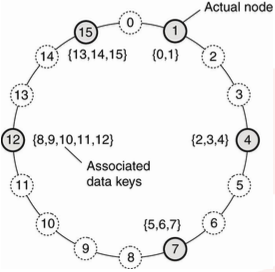
\includegraphics[width = .5\textwidth]{images/lezione2/chord.png}
\end{center}
I nodi tratteggiati nell'immagine indicano che non c'è un nodo effettivo, sono disponibili nel caso in cui entrasse un nuovo computer. \\
Quando entra un nuovo nodo si fa riallocazione delle risorse e si gestiscono i puntatori, in modo tale che un altro non punti più al 12, ma al 10 ad esempio e che il 10 abbia un puntatore al 12. Devo quindi gestire anche i link logici. 
\textbf{Esempio di applicazione} 
\begin{center}
    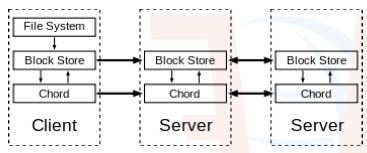
\includegraphics[width = .4\textwidth]{images/lezione2/applicazione-chord.png}
\end{center}
In questo esempio abbiamo una serie di server e un client che partecipa anche lui a chord. Hanno tutti un livello di middleware chord.\\
A livello del client abbiamo un'interfaccia al file system. \\
Il FS in realtà traduce le richieste (le mappa) in operazioni a basso livello sui blocchi (che sono distribuiti su tutte le macchine partecipanti). \\
Chord è usata per eseguire operazioni sui blocchi, per bilanciare la distribuzione dei blocchi e per trovare il server dove il blocco che serve è memorizzato.\\ LOOKUP è l'operazione che chord deve fare quando il FS chiede di accedere un blocco e occorre capire dov'è.

\paragraph{Distributed hash table}\mbox{}\\
Ciascuno dei nodi ha in esecuzione l'algoritmo che stiamo discutendo. Ciascuno ha anche una struttura dati "finger table" che è la tabella hash. Tante piccole parti di hash table sono distribuite nell'anello. \\
L'obbiettivo è rendere più efficiente la ricerca di una risorsa.\\
\begin{center}
    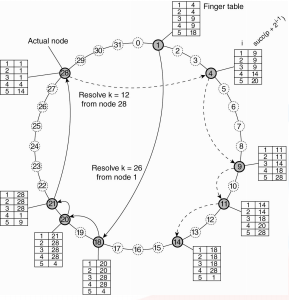
\includegraphics[width = .9\textwidth]{images/lezione2/DHT.png}
\end{center}
Ogni tabella ha 5 righe in quanto lo spazio di indirizzamento (nell'esempio) è di 5 bit.\\ 
Nella prima colonna, ogni riga fa riferimento al bit in questione, dunque da 1 a 5.
Il valore della seconda colonna è dato dalla formula \(succ(p + 2^{(i-1)})\), dove i è il valore della prima colonna e p è l'id del nodo.\\
Esempio: un client si collega al nodo 1 e chiede la risorsa 26. Viene guardata dunque la finger table del nodo 1 alla ricerca dell'elemento j (nella colonna di destra) tale per cui k (26) è \(\geq\), ma \(\leq\) del successivo (j+1). In questo caso il valore k (26) è maggiore di tutti i valori della finger table della colonna di destra e quindi viene presa in considerazione l'ultima riga della tabella. A questo punto viene eseguito un salto al nodo 18. Si esegue ancora la ricerca e in questa finger table si ferma alla seconda riga in quanto nella terza riga il valore della colonna di destra è \(>\) di k(26). Viene dunque eseguito un altro salto verso il nodo 20. Si esegue la stessa procedura e si salta al nodo 21. A questo punto, dato che già nella prima riga il valore è \(>\)
di k (26), si evince subito che la risorsa che si sta cercando risiede nel successore del nodo 21. Dunque la risorsa che si sta cercando (26) è contenuta nel nodo 28.

\paragraph{Strutturate: CAN (Content Addressable Network)}
\mbox{}\\Anche questo è basato su DHT (distributed hash table). Utilizza uno spazio cartesiamo d-dimensionale. \\
\begin{center}
    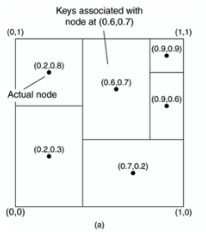
\includegraphics[width = .35\textwidth]{images/lezione2/CAN.png}
\end{center}
Questo spazio viene partizionato in nodi. In ogni rettangolo ci possono essere più punti. I punti sono associati ad un processo/nodo. I punti che si trovano al centro dell'area gestiscono tutte le risorse che verranno allocate, con delle funzioni che quindi mapperanno le risorse in uno spazio n-dimensionale, nell'area. \\
Quando arriva un altro nodo e viene allocato in un'area, quell'area viene divisa in due e le risorse di ciascun area sono associate ai rispettivi nodi. 

\paragraph{Limitazioni delle overlay strutturate}
Queste finger table vanno manutenute, con anche gli indirizzi e i puntatori. C'è un costo di overhead nel manutenere queste strutture. \\
Inoltre c'è il problema di organizzazione dei puntatori per essere resistente ai fallimento, occorre capire se un nodo è ancora online, posso fare un timeout, però questo non è banale, il problema potrebbe essere irrisolvibile. 

\paragraph{Non strutturate}
Hanno una struttura più semplice, senza DHT e senza manutenzione. \\
Si costruisce la rete con algoritmi randomizzati dove ogni nodo ha una vista parziale. \\
Ogni tanto i nodi vicini si scambiano informazioni sui nodi nuovi che hanno conosciuto, detti anche protocolli di gossiping. \\
Questo modo di scambiarsi i gossip ha delle componenti randomiche: si sceglie solo una percentuale a caso della view conosciuta da ciascuno. \\
C'è anche algoritmo di distribuzione delle risorse e anch'esso ha componente randomiche.  Possono essere diverse strategie. La ricerca non può dare garanzie fisse (upper bound, che trovi la risorsa, che ritorni più volte la stessa risorsa). L'effort di manutenzione è inferiore e migliora la scalabilità. La ricerca è limitata. Chiedono ai vicini per un numero limitato di hop o per un timeout temporale. 

\paragraph{Non strutturate: peer sampling}
La conoscenza locale dell'overlay è aggiornata basandosi sul servizio di peer sampling: i nodi si scambiano periodicamente le loro viste random e aggiornano le loro viste creando un nuovo campione random. Queste viste random definiscono un overlay network approssimativa

\paragraph{P2P: Strutturate vs Non strutturate}

% TABELLA MULTILINEA
\begin{table}[!ht]
    \centering
    \begin{tabular}{p{.12\textwidth}|p{.40\textwidth}|p{.35\textwidth}}
        \hline
         & Strutturate & Non Strutturate \\
        \hline
        Vantaggi & Garantisce di trovare gli oggetti (assumendo che esistano) e può offrire un margine a tempo e complessità a questa operazione. Overhead dei messaggi relativamente basso & Si auto-organizzano e sono resilienti dal fallimento dei nodi \\ 
        & &  \\
        Svantaggi & Ha bisogno di manutenzioni frequenti se la struttura è complessa, il che può essere costoso e difficile da ottenere, specialmente in ambienti molto dinamici & Non possono offrire garanzie di trovare l'oggetto. Si raggiunge un eccessivo overhead di messaggi che può influire sulla scalabilità \\ 
        \hline
    \end{tabular}
\end{table}

Ci sono anche soluzioni miste, ad esempio possiamo avere reti private/locali che funzionano in un certo modo con i regular peer e poi c'è un punto superpeer che a sua volta partecipa ad una rete a cui non partecipano i suoi sotto-peer.

\section{Architetture ibride}
BitTorrent è una rete peer to peer? Sì. È pura secondo definizione? Non proprio.\\ 
\begin{center}
    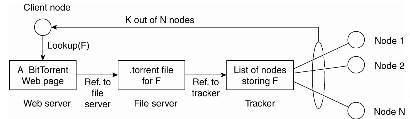
\includegraphics[width = .7\textwidth]{images/lezione2/Ibride.png}
\end{center}
Spesso c'è una componente iniziale che aiuta il resto del sistema a lavorare in modo centralizzato. Un client che vuole accedere ad una risorsa, all'inizio fa un lookup di f non direttamente ai nodi, ma a un webserver per trovare un .torrent, che è un file che non contiene il file, ma un riferimento ai tracker. \\
Il tracker è un nodo che coordina la distribuzione del file. \\
Quindi abbiamo all'inizio un'architettura client/server che va a identificare un riferimento, che porta ad un tracker e poi inizia la parte P2P vera e propria.


\section{Microservizi, Container e Servizi Cloud per SD}
\subsection{Microservizi}
Possono essere visti come una specie di raffinamento della distribuzione verticale: si cerca di andare a raffinare ancora di più anche all'interno dell'applicazione, isolando le singole funzionalità e rendendole indipendenti dalle altre. Questi microservizi devono interagire tra loro comunicando attraverso meccanismi leggeri, altrimenti l'overhead vanifica l'idea di separazione delle funzionalità per migliroare qualità. \\
Quindi si usano API REST o RPC. \\
I microservizi possono essere scritti in linguaggi di programmazione diversi, a seconda che una funzionalità sia meglio in un linguaggi piuttosto che un altro.\\ 
L'architettura a microservizi ha avuto successo perché permette di distribuire anche singoli servizi su macchine diverse, piuttosto che replicare tutto, a seconda delle necessità. \\
Potrei aver bisogno di replicare di più un componente piuttosto che un altro e così lo posso fare in modo più agile.
\begin{center}
    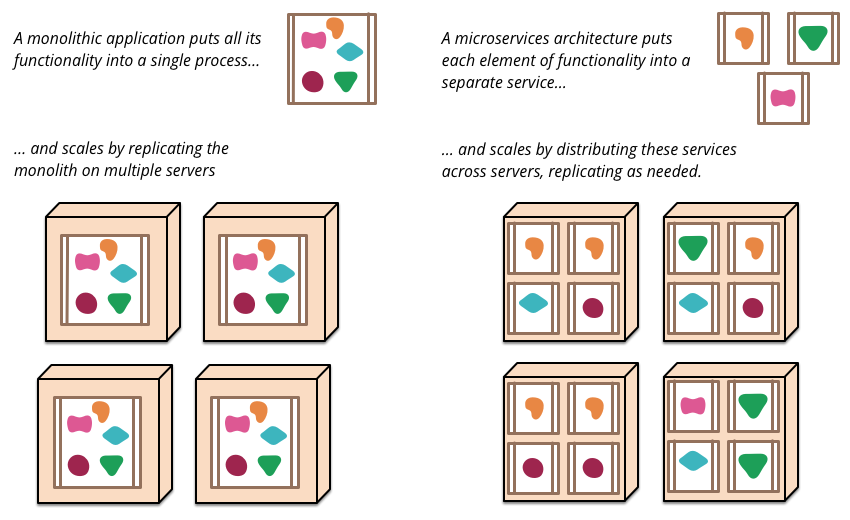
\includegraphics[width = .6\textwidth]{images/lezione2/sketch.png}
\end{center}

\subsection{Containers}
Sono un'astrazione a livello applicativo nelle quali l'idea è mettere insieme codice e dipendenze che il codice ha. L'obiettivo è quindi ospitare il codice dei microservizi e associare al microservizio anche le dipendenze di cui necessita, cercando di aumentare la portabilità e riducendo i problemi durante la fase di deployment. \\
Il container è l'analogo della VM. La VM è l'astrazione di una macchina fisica, mentre il container è l'astrazione a livello di una applicazione (tendenzialmente a livello di un microservizio).
\begin{center}
    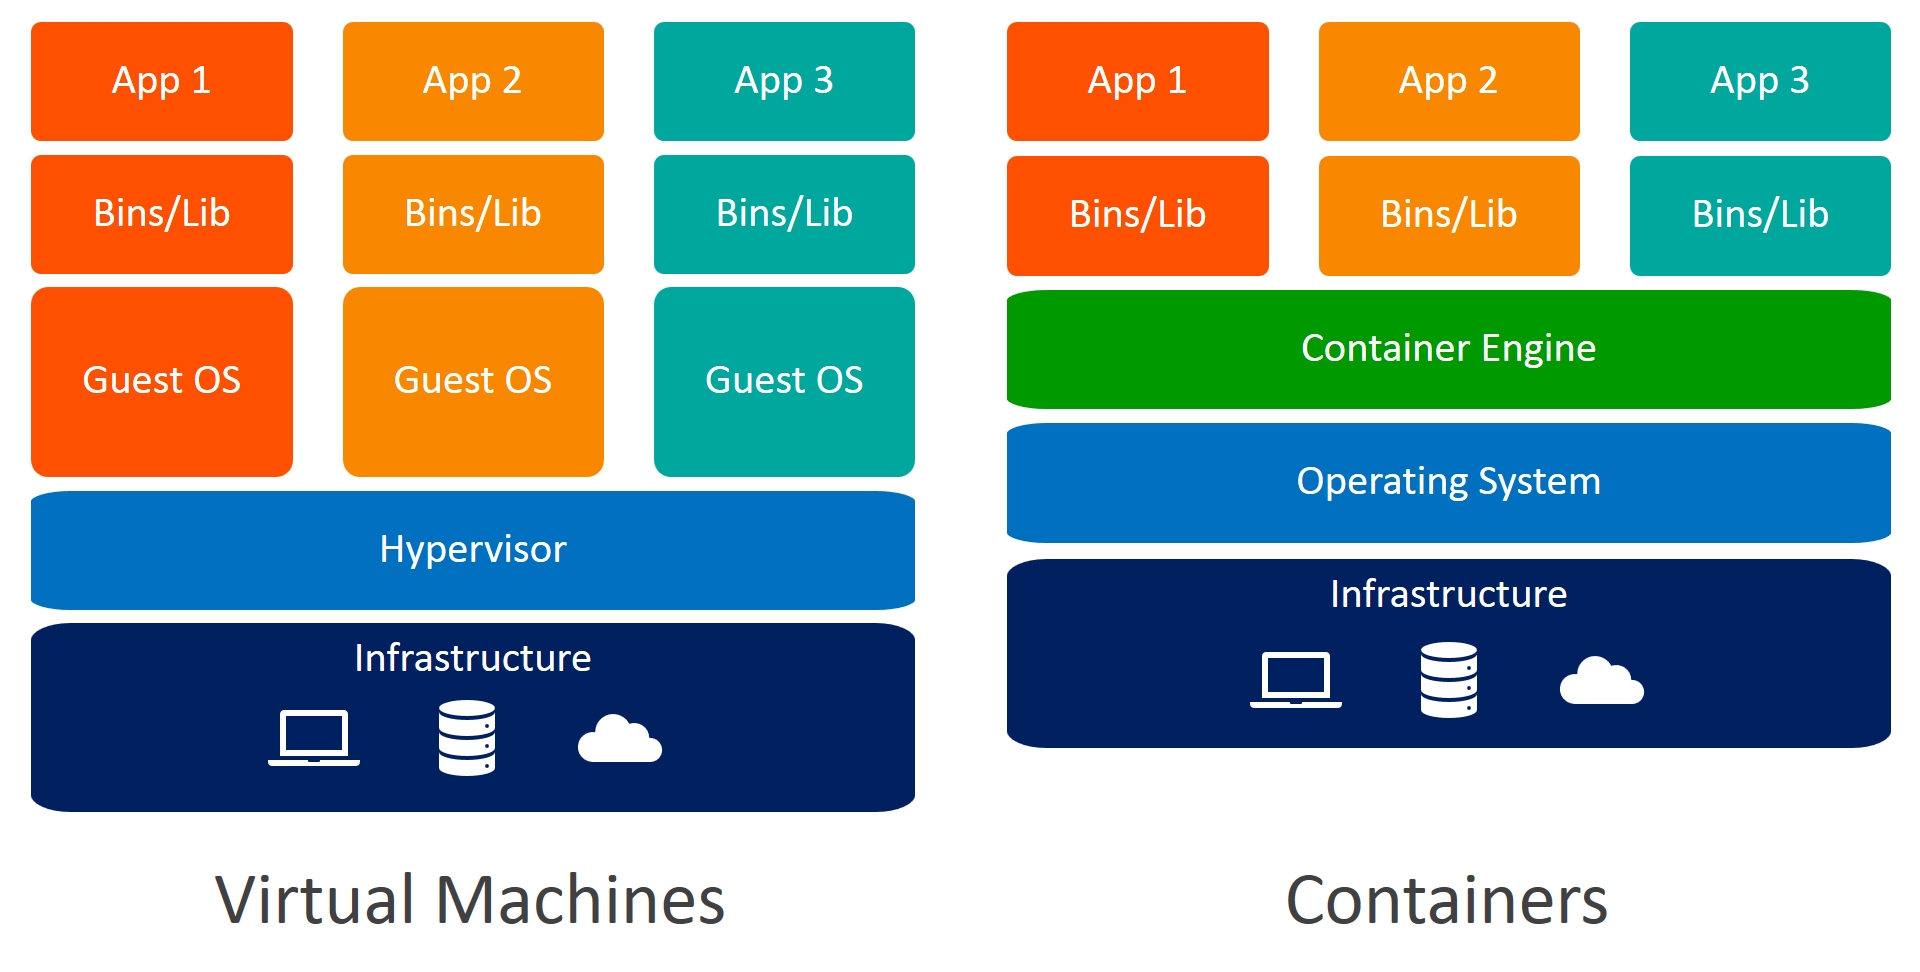
\includegraphics[width = .7\textwidth]{images/lezione2/containers-vs-virtual-machines.jpeg}
\end{center}
In ambito cloud è utilizzato l'approccio microservizi-container per distribuire su hw eterogeneo e distribuito in rete le funzionalità che vengono offerte come servizi cloud o SaaS. 


\subsection{Servizi Cloud per SD}
Sono insiemi di servizi costruiti su sistemi distribuiti e vengono applicati in:
\begin{itemize}
    \item Calcolo e comunicazione
    \item storage e DBMS
    \item identità e sicurezza
    \item management
\end{itemize}
Offrono diversi tipi di trasparenza.\\
I principali esponenti in questo campo sono:
\begin{itemize}
    \item Amazon AWS
    \item Google Cloud Platform
    \item Microsoft Azure
\end{itemize}

Alcuni esempi potrebbero essere:
\begin{itemize}
    \item Storage 
    \begin{itemize}
        \item Google Distributed File System (GFS, Colossus)
        \item Distributed RDBMS/NoSQL DBMS (Spanner)
    \end{itemize}
    \item Comunicazione
    \begin{itemize}
        \item Google PUB/SUB
    \end{itemize}
    \item Computazione e analisi di dati
    \begin{itemize}
        \item Google DataFlow
    \end{itemize}
\end{itemize}

Una delle problematiche del cloud è che è difficile fare il porting, appoggiandosi a diverse soluzioni specifiche di un fornitore di cloud. \\
Se usando i cloud si usano microservizi e container, questo favorisce la portabilità. \\
Quando si vuole coordinare comunicazioni e gestione di microservizi su container in un architettura a cluster diventa utile Kubernetes (evoluzione di Borg).





\begin{comment}
----------------------------------
Fabbio
Architettura software:
Principalmente software ma anche harware quando parliamo della distribuzione dei nodi (macchine, oggetti, servizi). IN alcuni casi in cluster (vicini) altri casi lontani.

Pattern di comunicazione:
-client-server
-event-bus (pub/sub)
-peer-to-peer

\textbf{architetture centralizzate:}
\textbf{client-server}, basato su un patter richiesta (client) risposta (server).
caching in client e server: i proxy fanno (anche) questo servizio.
multi-tier client-server (multilivello): divido le funzionalità lato server su un server separato (il server in generale è un processo, quindi non per forza sono su macchine diverse).

Distribuzione verticale: Diverse funzionalità gestite da diversi server
Distribuzione orizzontale: Stessa funzionalità gestita dallo stesso server
E' comune mettere insieme distribuzione verticale e orizzontale.

\textbf{Event Bus}:
C'è un componente centrale (broker) (server) che gestisce l'event bus. Nell'architettura ci sono dei publisher (client) e dei subscriver (client). Funzionalità simile allo stream, i subscriber rimangono in ascolto su di un canale in attesa della generazione di eventi mandati dai publisher. Sono asincroni, quindi i publisher inviano, se non c'è il subscriber in ascolto in quel momento il broker aspetta che lo sia e poi glie lo invia.

\textbf{Architetture decentralizzate:}
Modello peer-to-peer: Tutti i nodi in figura eseguono la stessa applicazione. Tutte le risorsse gestite dai peer sono fatte per essere condivise. Non c'è un coordinatore (un processo che fa da front-end del sistema).
Napster: primo sistema che ha dimostrato l'efficienza del P2P su larga scala (1999). Non era un P2P puro in quanto compare un napster server (c'è un indice). Però tutti i nodi eseguono tutti lo stesso codice, sono sia client che server. Ci sono degli indici centralizzati (per semplicità 1). Uno dei client vuole una risorsa, lo chiede al napster che non lo ha, ma ha la lista degli indirizzi di peer che lo hanno. Quindi contatta uno dei peer con i files e lo mette in comunicazione con chi ha chiesto la risorsa. Una volta ricevuto il file dice al napster server che ora anche lui ha il file e quindi chiede di aggiornare l'indice dei peer che lo posseggono.

Obiettivi P2P: Si vuole che le risorse siano bilanciate e quindi un po' di risorse in modo equo per tutti i peer. Limitare gli overhead.

Tre generazioni di P2P:
\textit{prima generazione}---
\textit{seconda generazione:}
BitTorrent efficiente perchè: ha una caratteristica fondamentale ovvero non bisogna scambiare la risorsa intera quindi vengono gestiti pezzetti di file. 
\textit{terza generazione:}
P2P Middleware - obiettivi:
Deve trovare facilmente le risorsa nel sistema, comunicare con la risorsa, aggiungere e togliere risorse e peer. Le risorse sono gestite da nodi, non sono i nodi.
Per farle si utilizza L'overlay networks per far comunicare i peer (rete logica sopra la rete fisica):
...
A cosa serve la rete logica:
-Routing overlay: si fa girare un software su tutti i nodi che fa il routing delle richieste da client (che sono anche esterni alla rete) agli host (nodi) che contengono le risorse di interesse. Il Routing è fatto a livello dell'applicazione (NON iso/osi). non è bassato su indirizzi ip ma identificatori globali. Un identificatore che univocamente identifica la risorsa. Il routing deve istradare verso uno dei peer che hanno la replica della risorsa. I protocolli di routing overlay devono occuparsi anche dell'aggiunta e della rimozione di risorse e dei peer.

Due tipi di overlay networks:
Le reti logiche di peer si differenziano in due tipi principali:
-\textbf{strutturata}: Più utilizzzata oggigiorno. Danno garanzie maggiori. C'è un algoritmo deterministico per creare la rete logica con il meccanismo espresso in tabelle di hashing. Ha lo scopo di raggiungere/togliere/mettere risorse/nodi.
-\textbf{non strutturata}: Usano algoritmi probabilistici. Ogni peer non sa esattamente dove si trova nella rete logica ma ha una vista parziale di alcuni altri peer. QUesta vista parziale si evolve nel tempo. Se si fa una richiesta a uno di questi nodi, questo peer (il nodo a cui si fa richiesta) o ha la risorsa o chiede ai peer che conosce se hanno la risorsa. Non è detto che la risorsa esiste nel sistema venga restituita.


Structured overlays: Chord
E' un sistema basato su DHT distributed hash table. 
Si fissa uno spazio di indirizzamento. Si definisce uno spazio per gli indirizzi fatto da 128 bit 160 bit (dipende dal istema). 
A ciascun nodo è associato un indirizzo. Un processo su una macchina in internet viene identificato da ip+porta. Actual node -> processo su una macchina che partecipa al sistema.
Se una risorsa ha id X, il nodo che la gestisce è quello con id minore maggiore di X. (se 3 è 4, se 5 è 7...)

Distributed hash tables:
CIascuno dei nodi ha una struttura dati (finger table -> tabella hash). L'obiettivo è quello di rendere più efficiente la ricerca di una risorsa. L'altezza della tabella è uguale al numero dei bit. 
left(i) = 2 --> right(p) = 4 + 2 ^ (i -1) = 4+2 = 6. Successore di 6 = [9]

Esercizio:
...

Structured overlays: CAN
Content addressbal network
Utilizza uno spazio cartesiano multi-dimensionale partizionato in nodi. I punti nella semplificazione b-dimensionale ci possono essere più punti per ogni regione e sono dati da due coordinate. I punti sono quelli assegnati ai nodi e in questo caso che sono al centro dell'area mapperanno le risorse in uno spazio n-dimensionale che verranno gestite dal nodo in questione.

Limitazioni delle structured overlays:
Costo per mantenere le strutture

Unstructured overlays:


Microservizi:
Raffinamento della distribuzione verticale. Isolare le singole funzionalità rendendole indipendenti dalle altre

Container:
astrazione a livello applicativo. Ospitare come codice microservizi e associare al microservizio anche le dipendenze di cui necessita.

----------------------------------
Simo
Architettura: 
si parla di architetture hw e sf, macchine distribuite geograficamente (possono essere cluster o altro)
L'architettura definisce le entità principali di un sistema. 
Entità che fanno parte: slide 3
Definisce i pattern di comunicazione: 
\begin{itemize}
    \item client/server
    \item event bus
    \item peer to peer
\end{itemize}

Un client può diventare server e poi tornare client. 
Tipi di architetture:
\begin{itemize}
    \item centralizzate
    \item decentralizzate
    \item ibride
\end{itemize}

Architetture centralizzate
Client server e event bus. 
Immagine slide 8
processo server in esecuzione su un nodo, processi client in esecuzione su altri nodi e possiamo avere più server. 
Ci sarà una richiesta da client (tramite istaurazione di un canale, come nelle socket). Il server deve gestire più richieste e deve rispondere. 

immagine slide 9
da sinistra a destra scorre il tempo. 
linea in nero marcato: processo in esecuzione
linea tratteggiata: processo non in esecuzione

il client nel pezzo tratteggiato va in wait.
Le frecce di richiesta/risposta sono oblique perché siamo in esecuzione su macchine distanti tra di loro (c'è un tempo che dobbiamo considerare che può dipendere da diversi fattori).

Quando progettiamo in un sistema client server ci poniamo il problema di cosa far eseguire lato client e cosa lato server. 
Esempi di modelli: immagine slide 10

In un'architettura client server c'è il caching attraverso un proxy. 
un client che ha fatto una richiesta in precedenza, perché andare a disturbare il server? si usa un proxy. 

Multi-tier
L'idea è quella di separare le funzionalità su più livelli. 

Distribuzione verticale vs orizzontale: 
modo per distribuire il carico. 
verticale: un server differente/nodo per ogni funzionalità
orizzontale: stessa funzionalità distribuita su più server. insieme di nodi che sono repliche dello stesso web server. 

È molto comune mettere insieme le due distribuzioni.

Event bus architecture
Il broker 
ci sono client chiamati publisher (serie di componenti sw) che comunicano il fatto che un evento si sia verificato (esempio deve comunicare le temperature in un edificio) comunicano su event bus (broker) che deve comunicare al subscriver tutto ciò che succede su un canale.

Architetture decentralizzate
Il modello più noto è il peer-to-peer.
immagine slide 21
Processi in esecuzione su nodi diversi del sistema distribuito. 
Ci sono risorse gestite da applicazioni su ogni peer. 
- All nodes have the same 
functional capabilities
- Designed so that each user 
contributes resources
- Operation does not depend 
on any centrally 
administered system (non c'è un processo che coordina, sono tutti alla pari)

Napster, primo file sharing system. Non era un P2P puro, ma molto vicino. 
Tutti i nodi hanno sia la funzionalità di client e server.
Ci sono indici centralizzati, il client vuole un file, manda la richiesta al server iniziale (non ha la risorsa il server), c'è una lista di indirizzi di peer che dovrebbe avere il file. Il peer usa uno di questi indirizzi e contatta il peer (che dovrebbe avere il file) ed ascolta come peer. Se ha il file invia il file al client.
Il client dice poi all'indice che anche lui ora ha il file. 

Uno dei principali problemi nei P2P è come distribuire le risorse.
obiettivi:
- Achieve load balancing while accessing data
- Ensuring availability avoiding overheads (disponibilità significa anche proteggersi da eventuali guasti)

3 generazioni di sistemi P2P:
\begin{itemize}
    \item First file sharing systems
    \item Protocols are refined to improve scalability, fault tolerance, anonymity
    \item P2P Middleware
\end{itemize}

Quali sono le cose più importanti che un middleware deve offrire?
- Deve riuscire a trovare facilmente le risrse nel sistema
- comunicare con le risorse
- questi sistemi sono dinamici, ci sono risorse che compaiono e scompaiono, stessa cosa per i peer. Quindi il middleware deve riuscire ad aggiungere e rimuovere risorse e peer

Per fare queste idee è di usare overlay networks: instaurare un pattern di comunicazione tra .....
overlay è una rete logica sopra rete fisica
la rete logica serve per fare in modo efficiente le 3 cose da offrire sopra elencate (middleware).
Sulla rete logica bisogna far girare un software (su tutti i nodi del sistema). Deve fare routing dai client agli host (nodi) che contengono le risorse che ci interessano. 
È un routing fatto a livello applicativo.
le risorse dovranno avere un identificatore che univocamente identifica la risorsa. 

Queste reti logiche di peer come si differenziano?
Due reti: 
- strutturata: danno garanzie maggiori. C'è un algoritmo deterministica per creare la rete logica 
- non strutturata: usano algoritmi probabilistici, randomizzati. ogni peer non sa dov'è nella rete logica ma ha una vista parziale che si evolve nel tempo

51:37 

----------

Omar

L'architettura:
-Definisce le entità principali del sistema.
-Definisce inoltre i pattern di comunicazione (vedremo client/server, event bus e P2P).
-Definisce come comunicano i processi tra di loro.
-Definisce il ruolo delle entità e come può evolversi durante l'esecuzione nel raggiungimento di un obbiettivo.
-Definisce anche come sono mappati sull'infrastruttura fisica.

Architetture centralizzate:
- Client-server
- Event Bus, segue pattern publish subscribe

Client server:
processo server in esecuzione su un nodo, processo client in esecuzione su altri nodi. Possono esserci anche più server. I pattern di comunicazione prevede una richiesta da parte del client (attraverso instaurazione canale, procedure call, ecc). Il server deve gestire più richieste e deve rispondere a tutti.
DISEGNINO
Da sinistra a destra scorre il tempo. La linea in nero marcato indica un processo in esecuzione. La linea dashed indica un processo che o non è in esecuzione o sta facendo altro (ad esempio il server potrebbe servire un altro client e il client va in wait in attesa della risposta). Le frecce di richiesta/risposta sono oblique perché c'è sempre un delay di comunicazione, quindi c'è un tempo da considerare.
Nella progettazione client/server occorre capire cosa eseguire lato client e cosa lato server. Ci sono diverse possibili scelte, che possono scaricare compiti al client o scaricare al server nei due estremi.
Possibile anche usare sistemi di caching. I proxy fanno anche questo servizio. Se una richiesta client eseguita in precedenza e il proxy ritiene che la risposta sia ancora valida, restituisce la stessa risposta (?).
Architetture multi-livello: lato server divido funzionalità (in quello a 3 livelli) tra application server e database server (sono processi diversi, non è detto che siano macchine diverse).
Distribuzione verticale: spesso nodi diversi. Server (Processi) diversi per ogni funzionalità.
Distribuzione orizzontale: stessa funzionalità distribuita (replicata) su più server diversi.
È molto comune mettere insieme distribuzione orizzontale e verticale. Load balancer gestisce le richieste del client e lato server possiamo avere una distribuzione verticale con una distribuzione orizzontale per qualche funzionalità (?).
Ogni volta che c'è una distrubuzione orizzontale c'è un load balancer.

Event Bus:
C'è un componente centrale Event Bus. Broker componente software che gestisce l'event bus. Ci sono dei client (chiamati publisher) che comunicano il fatto che un evento si sia verificato. Dall'altra parte c'è un altro "client" (chiamato subscriber) che fa una subscription specifica a ricevere le informazioni da un canale (?). Il compito del broker sarà incaricato di comunicare al subscriber interessati agli eventi di un certo tipo tutto quello che succede su quel canale. In questo modo viene reso asincrono, perché non è detto che il subscriber sia collegato in quel momento (?).

Architetture decentralizzate:
- peer to peer:
Abbiamo un certo numero di peer. Ci sono delle risorse che sono gestite da applicazioni su ciascuno di questi peer. In un peer to pper puro tutti i nodi eseguono la stessa applicazione, hanno quindi stessa capacità funzionale. Le risorse gestite dai vari peer sono fatte per essere in qualche modo condivise. Non c'è un coordinatore (load balancer, ad esempio, quindi un processo che fa da frontend del sistema), sono tutti alla pari. 
Esempio Napster: primo sistema che ha dimostrato utilità e efficacia di un sistema distribuito su larga scala per lo scambio di risorse che osno file. Piu di 20 anni fa. È stato chiuso per questioni di copyright. Questo sistema non era peer to peer puro. C'è un napster server che mantiene un index. Tutti i nodi hanno sia funzionalità di client e di server ed eseguono tutti lo stesso codice, tranne appunto i server "direcory". Ci sono indici centralizzati. Un client vuole un certo file, manda richiesta al server iniziale che risponde con una lista di indirizzi di peer che dovrebbero avere quel file. Il peer a questo punto usa uno di questi indirizzi e contatta un altro peer, che si comporta da server. Se ha il file lo restituisce al client (quello che fa la richiesta) come risposta. Il client dice all'indice di aggiornarsi che anche lui adesso ha il file. Viene quindi reso disponibile il file su più punti della rete P2P.
Uno dei problemi principali è come distribuire le risorse. Gli obiettivi nel distribuire sono:
-raggiungere load balancing quando si accede ai dati, migliore quindi performance
-vogliamo anche assicurare disponibilità, proteggersi quindi da guasti
-evitare troppi overhead
Prima generazione: napster
Dopodiché qualcuno si è concentrato sul migliorare scalabilità, fault tolerance o anonimità: Gnutella (tentativo di fare un sistema puro che funziona su larga scala, non usa directory service completi. Ha indici parziali e distribuiti), FreeNet (fornire file sharing che garantisse anonimità), bitTorrent (particolarmente efficiente, per una caratteristica fondamentale: non viene scambiata la risorsa intera. Vengono gestiti diversi pezzetti di file).
Dopodiché c'è un'altra generazione P2P Middleware: viene creato un sistema che è una specie di middleware per gestire in modo didstirbuito e decentralizzato delle risorse.

P2P Middleware deve garantire:
- In modo trasparente
    - localizzare e comunicare con una risorsa
    - aggiungere e rimuovere risorse
    - agigungere e rimuovere peer (far entrare e uscire)
Per farlo si costruisce degli overlay networks. Rete logica/irtuale costruita sopra la vera rete (fisica) che collega i peer. Criteri di ottimizzazione: scalabilità, load blancing, far comunicare quelli vicini (minore latenza), sicurezza e anonimità. Questa rete logica consente di effettuare in modo efficiente le cose suddette. 
Sulla rete logica viene seguito il routing delle richieste (a livello applicazione) da client magari anche esterni alla rete agli host/nodi che contengono le risorse che ci interessano). Non è il routing del protocollo IP, è routing a livello di applicazione. È pasato non su indirizzi IP, ma su identificatori globali. Le risorse hanno identificatori globali nel sistema distribuito. Il routing deve instradare verso uno dei peer che hanno una replica della risosa (quindi possono averla più di uno). I protocolli di routing overlay devono anche occuparsi di inserire e rimuovere nodi e oggetti. Questo algoritmo è installato su tutti i nodi del sistema. 

Due tipi di overlay networks:
- strutturate
    - più utilizzate oggi. Danno garanzie maggiori. In queste reti c'è un algoritmo deterministico con strutture dati particolari per cerare questa rete logica ( spesso viene gestita tramite tabelle di hashing).
- non strutturate
    - usano algoritmi probabilistici/randomizzati. Ogni peer non sa esattamente dov'è nella rete logica. Ha una vista parziali di alcuni altri peer che si evolve nel tempo. Siccome è parziale, nel momento in cui un client fa una richiesta a uno di questi peers, o ha la risosa, o chiede ai peer che conosce. Non c'è garanzia che la conosca. Viene richiesto man mano. Si cerca di ricostruire e aggiornare le partial view.
    
Strutturate: chord
Algoritmi abbastanza complicati. Articolo che spiega in dettaglio nel materiale. 
Sistema  basato su DHT distributed hash table, come la maggior parte di sistemi con overlay strutturate. Per prima cosa si fissa uno spazio di indirzzamento, tipicamente fatto di 128-160bit. Nell'esempio 16 bit. A ciascun nodo è associato un indirizzo nello spazio. Identifico un processo sulla macchina attraverso una hashing function che prende ip e porta e produce un'indirizzo in questo spazio (?). Gli actual node corrispondono ad un processo sulla macchina che partecipa al sistema. Lo stesso spazio di indirzzamento è utilizzato per le risorse. Ciascuna risorsa avrà una chiave. L'hashing della chiave in questo spazio darà un certo numero. Il discorso dell'hashing da garanzia di distribuire in maniera uniforme nello spazio. Un dato con chiave K viene mappato nel nodo con il più piccolo ID >= k. La funzione LOOKUP o "successore", data la risorsa restituisce quale nodo la gestisce. I nodi trattegiati indicano che non c'è un nodo effettivo, sono disponibili nel caso in cui entrasse un nuovo computer. Quando entra si fa riallocazione delle risorse e gestire i puntatori, in modo tale che un altro non punti più al 12, ma al 10 ad esempio e che il 10 abbia un puntatore al 12. Devo quindi gestire anche i link logici. La cosa più difficile è fare efficientemente il LOOKUP. Una soluzione un po' furba è trovare un algoritmo che abbia complessità logn del numero dei nodi.
Esempio di applicazioni: una serie di server e un client che aprtecipa anche lui a chord. Hanno livello di middleware chord. POiu c'è un interfaccia di filesystem nel client, come se avesse l'intero filesystem. Il FS in realtà traduce le richieste in operazioni sui blocchi. I blocchi sono distribuiti. Le risorse in questo caso sono i blocchi. Le operazioni sui blocchi sono fatte consultando chord per opi usare overlay e tutto quanto. CHord bilancia la distribuzione dei blocchi e trovare il server dove il blocco che serve è memorizzato. LOOKUP è l'operazione che chord deve fare quando FS chiede di accere un blocco e occorre capire dov'è.
Distributed hash table: ciascuno dei nodi ha in secuzione l'algoritmo che stiamo discutendo. Ciascuno ha anche una struttura dati "finger table" che è la tabella hash. Tante piccole parti di hash table osno distribuite nell'anello. L'obbiettivo è rendere più efficiente la ricerca di una risorsa. In ogni tablelina colonna 1 è 12345 perché lo spazio di indirzzamento è 5 bit. Dunque l'altezza della tabella è uguale al numero di bit. Nella seconda colonna c'è succ(p + 2^(i-1)), dove i è il valore della prima colonna. p è l'id del nodo. Esempio: client si collega a nodo 1 e chiede risorsa 26. Guarda la tabella, identifica l'elemento j per cui k è >=, ma <= del successivo (j+1). Va quindi fino in fondo perché K = 26 è maggiore di tutti i numeri. A questo punto fa quindi il salto a 18. Guarda ancora la tabella si ferma 2-20 poiché 3-28 è maggiore e così via. Nella tabella del 21 ottengo subito una riga più grande, quindi la risorsa è sul successore di questo, quindi il 28.

Strutturate: CAN Content Addressable Network
Anceh questo è basato su DHT (distributed hash table). Utilizza uno spazio cartesiamo d-dimensionale. Questo spazio viene partizionato in nodi. In ogni rettangolo ci possono essere più punti. I punti sono associati ad un processo/nodo. I punti che si trovano al centro dell'area gestiscono tutte le risorse che verranno allocate, con delle funzioni che quindi mapperanno le risorse in uno spazio n-dimensionale, nell'area. Quando arriva un altro nodo e viene allocato in un'area, quell'area viene divisa in due e le risorse di ciascun area sono associate ai rispettivi nodi. 

Queste finger table vanno manutenute, con anche gli indirizzi e i puntatori. C'è un costo di overhead nel manutenere queste strutture. Inoltre c'è il problema di organizzazione dei puntatori per essere resistente ai fallimento, occore capire se un nodo è ancora online, posso fare un timeout, però questo non è banale, il problema potrebbe essere irrisolvibile (?). 

Non strutturate:
Struttura più semplice, senza dht e senza manutenzione. Si costruisce la rete con algoritmi randomizzati. Ogni nodo ha una vista parziale. Ogni tanto i nodi vicini si scambiano informazioni sui nodi nuovi che hanno conosciuto, detti anche protocolli di gossiping. Questo modo di scambiarsi i gossip ha delle componenti randomiche: si sceglie solo una percentuale a caso della view conosciuta da ciascuno. C'è anche algoritmo di distribuzione delle risorse, anch'esso ha componente randomiche. Possono essere diverse strategie. La ricerca non può dare garanzie fisse (upper bound, che trovi la risorsa, che ritorni più volte la stessa risorsa). L'effort di manutenzione è inferiore e migliora la scalabilità. La ricerca è limitata. Chiedono ai vicini per un numero limitato di hop o per un timeout temporale. 

Non strutturate: peer sampling

...

Strutturate vs non struttureate:
I vantaggi di strutturate sono garanzie di trovare risorse e efficienza nelle operazioni. Overhead dei messaggi relativamente basso. Si risparmiano messaggi rispetto ad un flooding della rete, il quale è uno svantaggio dell'unstructured (?). Vantaggi nella non strutturata è che se un nodo sparisce dalla rete, trova qualche altro nodo per fare la richiesta, ma non c'erano strutture particolari. Se qualceh peer aveva un puntatore a questo, con un timeout capisce che non c'è più. Non c'è da fare manutenzione particolare. Svantaggi strutturati: occorre mantenere strutture dati, quindi ci sono costi associati.

Ci sono anche soluzioni miste, ad esempio possiamo avere reti private/locali che funzionano in un certo modo con i regular peer e poi c'è un punto superpeer che a sua volte partecipa ad una rete a cui non partecipano i suoi sottopeer.

BitTorrent è una rete peer to peer? Sì. È pura seocndo definizione? Nì. Spesso c'è una componente iniziale che aiuta il resto del sistema a lavorare in modo centralizzato. UN client che vuole accedere ad una risorsa, all'inizio fa un lookup di f non direttamente ai nodi, ma a un webserver per trovare un .torrent, che è un file che non contiene il file, ma un riferimento ai tracker. Il tracker è un nodo che coordina la distribuzione del file. Quindi abbiamo all'inizio un'architettura client/server che va a identificare ad un riferimento, che porta ad un tracker e poi inizia la parte P2P vera e propria.

Microservizi: 
Una specie di raffinamento della distribuzione verticale. Andare a raffinare ancora di più anche all'interno dell'aplicazione isolando le singole funzionalità e rendendole indipendenti dalle altre. Questi microservizi devono interagire tra loro comunicando attraverso meccanismi leggeri, altrimenti l'overhead vanifica l'idea di separazione delle funzionalità per migliroare qualità. Quindi usano api rest o rpc. Possono essere scritti in linguaggi di programmazione diversi, a seconda che una funzionalità sia meglio in un linguaggi piuttosto che un altro. 
Architettura microservizi ha avuto successo perché posso distribuire anche singoli servizi su macchine diverse, piuttosto che replicare tutto, secondo necessità. POtrei aver bisogno di replicare di più un componente piuttosto che un altro e così lo posso fare in modo più agile.

Containers:
Sono un'astrazione a livello applicativo. L'idea è mettere insieme codice e dipendenze che il codice ha. L'idea è quindi di ospitare come codice dei microservizi e associare al microservizio anche le dipendeze di cui necessita. Il container è l'analogo della VM. La VM è l'astrazione di una macchina fisica, mentre il container è l'astrazione a livello di una applicazione. Tendenzialmente a microservizio. È possibile anche condividere dipendenze tra container (?).

In ambito cloud è utilizzato l'approccio (microservizi e container) per distribuire su hw eterogeneo e distribuito in rete le funzionalità che vengono offerte come servizio cloud o SaS. 

Storage:
-sono filesystem distribuiti (GFS...)
-Databse relazione distribuiti
Comunicazione:
-publish/subscribe
processing di stream di dati:
...

Una delle problematiche del cloud è difficile fare il porting, appoggiandosi a diverse soluzione specifiche di un fornitore di cloud. Se usando i cloud si usano microservizi e container, questo favorisce la portabilità. C'è un problema di locking, quindi.
Quando si vuole coordinare comunicazioni e gestione di microservizi su container in un architettura a cluster diventa utile kubernates, evoluzione di Borg (?).



\end{comment}